\chapter{Layers in NN models}

\begin{itemize}
    \item \url{https://pytorch.org/docs/stable/nn.html#linear-layers}
    \item \url{https://www.tensorflow.org/api_docs/python/tf/keras/layers}
\end{itemize}

%%%%%%%%%%%%%%%%%%%%%%%%%%%%%%%%%%%%%%%%%%%%%%%%%%%%%%%%%%%%

\section{Linear Layer/ Dense Layer \cite{pytorch-Linear,gfg-convolutional-neural-network-cnn-in-machine-learning}}\label{nn: Linear Layer/ Dense Layer}

\begin{itemize}
    \item These layers are responsible for making predictions based on the high-level features learned by the previous layers. 
    
    \item They connect every neuron in one layer to every neuron in the next layer.
    
    \item Applies a linear transformation to the incoming data: $\mathbf{y=xA^\top+b}$.
\end{itemize}


%%%%%%%%%%%%%%%%%%%%%%%%%%%%%%%%%%%%%%%%%%%%%%%%%%%%%%%%%%%


\section{Convolution Layer \cite{gfg-convolutional-neural-network-cnn-in-machine-learning}}\label{nn: Convolution Layer}

\[
   \displaystyle n_{out} = \left[ \frac{n_{in} + 2p - k}{s} \right] + 1
\]

\begin{itemize}
    \item These layers apply convolutional operations to input images, using filters (also known as kernels) to detect features such as edges, textures, and more complex patterns. 
    
    \item Convolutional operations help preserve the spatial relationships between pixels.
\end{itemize}

%%%%%%%%%%%%%%%%%%%%%%%%%%%%%%%%%%%%%%%%%%%%%%%%%%%%%%%%%%%%

\section{Pooling Layer \cite{gfg-convolutional-neural-network-cnn-in-machine-learning}}\label{nn: Pooling Layer}

\[
   \displaystyle n_{out} = \left[ \frac{n_{in} - k}{s} \right] + 1
\]

\begin{itemize}
    \item Pooling layers \textbf{downsample} the spatial dimensions of the input, reducing the computational complexity and the number of parameters in the network. 
    
    \item Max pooling is a common pooling operation, selecting the maximum value from a group of neighboring pixels.

\end{itemize}

%%%%%%%%%%%%%%%%%%%%%

\subsection{Max Pooling \cite{gfg-cnn-introduction-to-pooling-layer}}\label{cnn: Max Pooling}

\begin{itemize}
    \item Max pooling is a pooling operation that selects the \textbf{maximum element} from the region of the feature map covered by the filter. 
    
    \item The output after max-pooling layer would be a feature map containing the \textbf{most prominent features} of the previous feature map.
\end{itemize}

%%%%%%%%%%%%%%%%%%%

\subsection{Average Pooling \cite{gfg-cnn-introduction-to-pooling-layer}}\label{cnn: Average Pooling}
\begin{itemize}
    \item Average pooling computes the \textbf{average of the elements} present in the region of feature map covered by the filter.
    
    \item Average pooling gives the average of features present in a patch.
\end{itemize}

%%%%%%%%%%%%%%%%%%

\subsection{Global Pooling \cite{gfg-cnn-introduction-to-pooling-layer}}\label{cnn: Global Pooling}
\begin{itemize}
    \item Global pooling reduces each channel in the feature map to a single value.
    
    \item Thus, an $n_h \times n_w \times n_c$ feature map is reduced to $1 \times 1 x nc$ feature map. 

    \item This is equivalent to using a filter of dimensions $n_h \times n_w$ i.e. the dimensions of the feature map.
\end{itemize}

\begin{table}[h]
    \begin{minipage}[t]{0.32\linewidth}
        \begin{figure}[H]
            \centering
            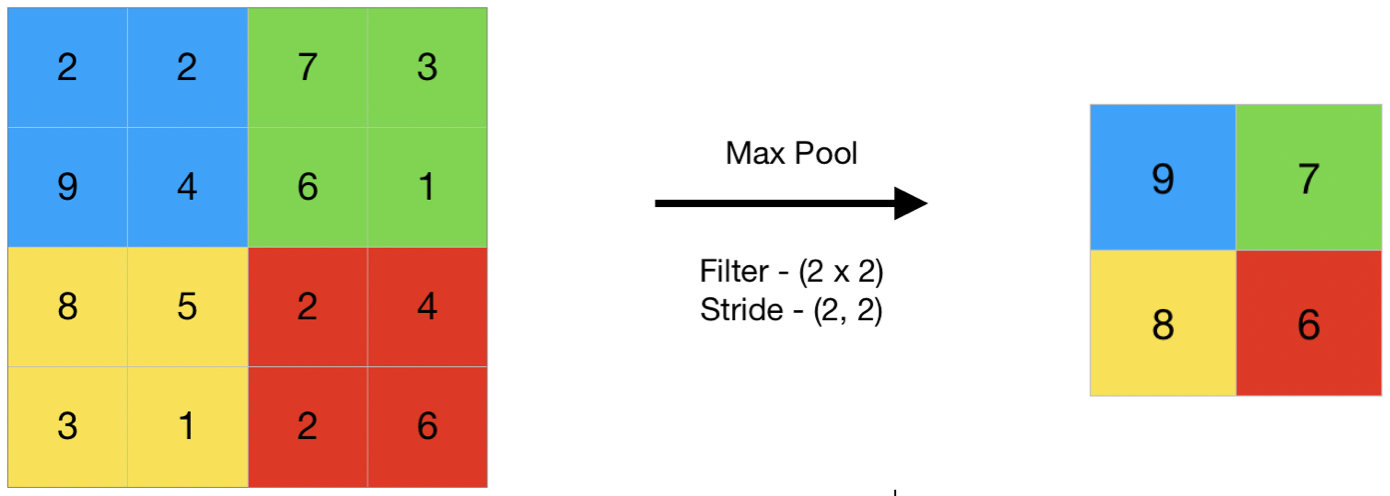
\includegraphics[width=\linewidth, height=4cm, keepaspectratio]{Pictures/convolutional-neural-network/pooling-max.png}
            \caption{Max Pooling}
        \end{figure}
    \end{minipage}
    \hfill
    \begin{minipage}[t]{0.32\linewidth}
        \begin{figure}[H]
            \centering
            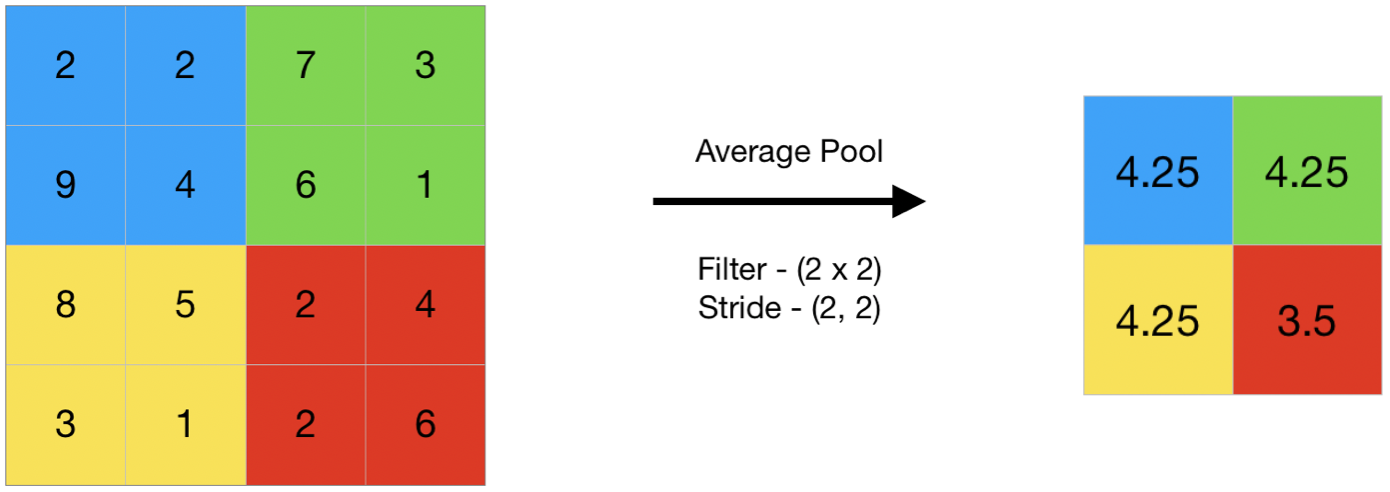
\includegraphics[width=\linewidth, height=4cm, keepaspectratio]{Pictures/convolutional-neural-network/pooling-average.png}
            \caption{Average Pooling}
        \end{figure}
    \end{minipage}
    \hfill
    \begin{minipage}[t]{0.32\linewidth}
        \begin{figure}[H]
            \centering
            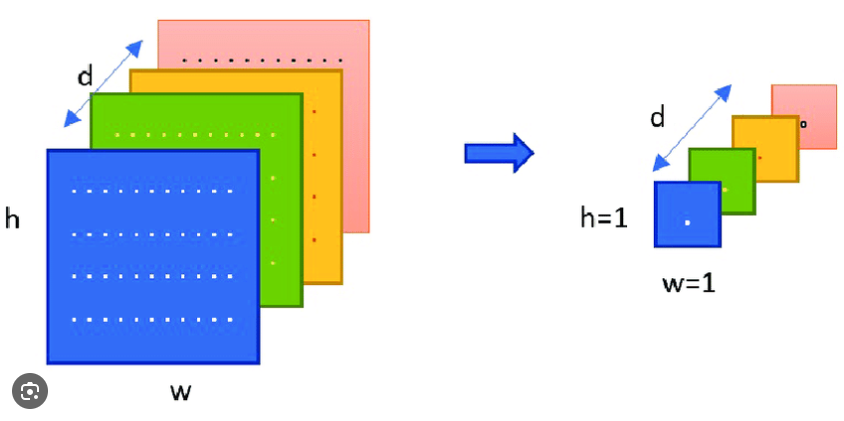
\includegraphics[width=\linewidth, height=4cm, keepaspectratio]{Pictures/convolutional-neural-network/pooling-global.png}
            \caption{Global Pooling}
        \end{figure}
    \end{minipage}
\end{table}

%%%%%%%%%%%%%%%%%%%%%%%%%%%%%%%%%%%%%%%%%%%%%%%%%%%%%%%%%%%%%%

\section{Dropout Layer \cite{gfg-dropout-in-neural-networks,medium/towardsdatascience.com/dropout-in-neural-networks-47a162d621d9}}\label{nn: Dropout Layer}

\begin{figure}[H]
    \centering
    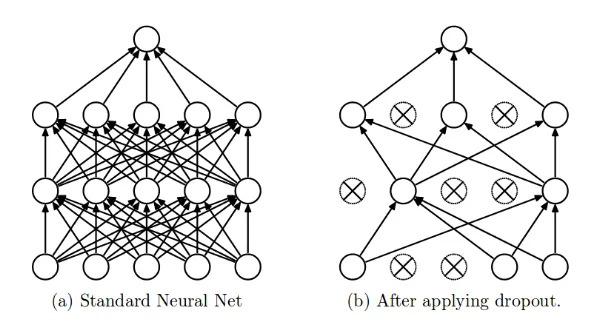
\includegraphics[width=\linewidth, height=3.5cm, keepaspectratio]{Pictures/layers/dropout.jpg}
    \caption{Dropout Layer \cite{medium/towardsdatascience.com/dropout-in-neural-networks-47a162d621d9}}
\end{figure}

\begin{itemize}
    \item The term “dropout” refers to dropping out the nodes (input and hidden layer) in a neural network. 
    
    \item All the forward and backwards connections with a dropped node are temporarily removed, thus creating a new network architecture out of the parent network. 
    
    \item The nodes are dropped by a dropout probability of p.

    \item In every iteration, you will work on a smaller neural network than the previous one and therefore, it approaches \textbf{regularization}.

    \item Dropout helps in \textbf{shrinking} the squared norm of the weights and this tends to a reduction in overfitting.
\end{itemize}


%%%%%%%%%%%%%%%%%%%%%%%%%%%%%%%%%%%%%%%%%%%%%%%%%%%%%%%%%%%%%%


\section{Flatten Layer \cite{gfg/what-is-a-neural-network-flatten-layer}}\label{Flatten Layer}

\begin{itemize}
    \item A neural network flatten layer is used to convert the multi-dimensional output from the previous layer into a \textbf{one-dimensional array}, typically before feeding it into a fully connected layer for further processing.

    
\end{itemize}


%%%%%%%%%%%%%%%%%%%%%%%%%%%%%%%%%%%%%%%%%%%%%%%%%%%%%%%%%%%%%%

\section{Activation Layer}
\textbf{SEE}: \fullref{chapter: Activation Functions}
















































































